\documentclass[12pt]{article}

\usepackage{fullpage}
\usepackage[round]{natbib}
\usepackage{multirow}
\usepackage{booktabs}
\usepackage{graphicx}
\usepackage{hyperref}

\hypersetup{
    bookmarks=true,         % show bookmarks bar?
      colorlinks=true,       % false: boxed links; true: colored links
    linkcolor=red,          % color of internal links (change box color with linkbordercolor)
    citecolor=green,        % color of links to bibliography
    filecolor=magenta,      % color of file links
    urlcolor=cyan           % color of external links
}
\newcounter{acnum}
\newcommand{\actheacnum}{AC\theacnum}
\newcommand{\acref}[1]{AC\ref{#1}}

\newcounter{ucnum}
\newcommand{\uctheucnum}{UC\theucnum}
\newcommand{\uref}[1]{UC\ref{#1}}

\newcounter{mnum}
\newcommand{\mthemnum}{M\themnum}
\newcommand{\mref}[1]{M\ref{#1}}

%% Comments
\newif\ifcomments\commentstrue

\ifcomments
\newcommand{\authornote}[3]{\textcolor{#1}{[#3 ---#2]}}
\newcommand{\todo}[1]{\textcolor{red}{[TODO: #1]}}
\else
\newcommand{\authornote}[3]{}
\newcommand{\todo}[1]{}
\fi

\newcommand{\wss}[1]{\authornote{magenta}{SS}{#1}}

\begin{document}

\title{Module Guide for Open Source 
  Game Physics Library} 
\author{Alex Halliwushka}
\date{\today}
	
\maketitle

\tableofcontents

\newpage

\section{Introduction}

Decomposing a system into modules is a commonly accepted approach to developing
software.  A module is a work assignment for a programmer or programming
team~\citep{ParnasEtAl1984}.  In the best practices for scientific computing,
\citet{WilsonEtAl2013} advise a modular design, but are silent on the criteria
to use to decompose the software into modules.  We advocate a decomposition
based on the principle of information hiding~\citep{Parnas1972a}.  This
principle supports design for change, because the ``secrets'' that each module
hides represent likely future changes.  Design for change is valuable in SC,
where modifications are frequent, especially during initial development as the
solution space is explored.  

Our design follows the rules laid out by \citet{ParnasEtAl1984}, as follows:
\begin{itemize}
\item System details that are likely to change independently should be the
  secrets of separate modules.
\item Each data structure is used in only one module.
\item Any other program that requires information stored in a module's data
  structures must obtain it by calling access programs belonging to that module.
\end{itemize}

After completing the first stage of the design, the Software Requirements
Specification (SRS), the Module Guide (MG) is developed~\citep{ParnasEtAl1984}. The MG
specifies the modular structure of the system and is intended to allow both
designers and maintainers to easily identify the parts of the software.  The
potential readers of this document are as follows:

\begin{itemize}
\item New project members: This document can be a guide for a new project member
  to easily understand the overall structure and quickly find the
  relevant modules they are searching for.
\item Maintainers: The hierarchical structure of the module guide improves the
  maintainers' understanding when they need to make changes to the system. It is
  important for a maintainer to update the relevant sections of the document
  after changes have been made.
\item Designers: Once the module guide has been written, it is can be used to
  check for consistency, feasibility and flexibility. Designers can verify the
  system in various ways, such as consistency among modules, feasibility of the
  decomposition, and flexibility of the design.
\end{itemize}

The rest of the document is organized as follows. Section
\ref{SecChange} lists the anticipated and unlikely changes of the software
requirements. Section \ref{SecMH} summarizes the module decomposition that
was constructed according to the likely changes. Section \ref{SecConnection}
specifies the connections between the software requirements and the
modules. Section \ref{SecMD} gives a detailed description of the
modules. Section \ref{SecTM} includes two traceability matrices. One checks
the completeness of the design against the requirements provided in the SRS. The
other shows the relation between anticipated changes and the modules. Section
\ref{SecUse} describes the use relation between modules.

\section{Anticipated and Unlikely Changes} \label{SecChange}

This section lists possible changes to the system. According to the likeliness
of the change, the possible changes are classified into two
categories. Anticipated changes are listed in Section \ref{SecAchange}, and
unlikely changes are listed in Section \ref{SecUchange}.

\subsection{Anticipated Changes} \label{SecAchange}

Anticipated changes are the source of the information that is to be hidden
inside the modules. Ideally, changing one of the anticipated changes will only
require changing the one module that hides the associated decision. The approach
adapted here is called design for
change. %Anticipated changes are numbered by \textbf{AC} followed by a number.

\begin{description}
\item[\refstepcounter{acnum} \actheacnum \label{acHardware}:] The specific
  hardware on which the software is running.
\item[\refstepcounter{acnum} \actheacnum \label{acBody}:] The data structure of the
physical properties of an object such as the object's mass, position and velocity.
\item[\refstepcounter{acnum} \actheacnum \label{acShape}:] The data structure of the
surface properties of an object such as the object's friction and elastiicity
\item[\refstepcounter{acnum} \actheacnum \label{acCollision}:] The data structure of the 
collision such as the objects that collide and their mass. 
\item[\refstepcounter{acnum} \actheacnum \label{acConstraint}:] The data structure 
of how the bodies are constrained, such as the bodies that are constrained and the
type of constraint. 
\item[\refstepcounter{acnum} \actheacnum \label{acSpace}:] How all the rigid
bodies, shapes, and constraints interact together
\item[\refstepcounter{acnum} \actheacnum \label{acControl}:] How the overall
  control of the simulation is orchestrated.
\item[\refstepcounter{acnum} \actheacnum \label{acSeqDS}:] The implementation
  for the sequence (array) data structure.
  
\item[\refstepcounter{acnum} \actheacnum \label{acLinkDS}:] The implementation
  for the linked (tree) data structure.
  
\item[\refstepcounter{acnum} \actheacnum \label{acAssDS}:] The implementation
  for the associative (hash table) data structure.
  
\item[\refstepcounter{acnum} \actheacnum \label{acSolver}:] The algorithm used
  for solving collisions.
\item[\refstepcounter{acnum} \actheacnum \label{acQuery}:] The algorithm used
  for spatial queries.
\end{description}

\subsection{Unlikely Changes} \label{SecUchange}

The module design should be as general as possible. However, a general system is
more complex. Sometimes this complexity is not necessary. Fixing some design
decisions at the system architecture stage can simplify the software design. If
these decision should later need to be changed, then many parts of the design
will potentially need to be modified. Hence, it is not intended that these
decisions will be changed. 

% As an example, the ODEs for the temperature and the
%energy equations are assumed to follow the structure given in the SRS; that is,
%even if they need to be modified, the modifications should be possible by
%changing how the input parameters are used in the definition.  If new parameters
%are needed, this will mean a change to both the input parameters module, the
%calculation module and the output module.

\begin{description}
\item[\refstepcounter{ucnum} \uctheucnum \label{ucIO}:] Input/Output devices
  (Input: Keyboard and/or mouse, Output: Memory and/or Screen).
\item[\refstepcounter{ucnum} \uctheucnum \label{ucOutput}:] Output data are
  displayed to the output device.
\item[\refstepcounter{ucnum} \uctheucnum \label{ucGoal}:] The goal of the system
  is to simulate the interactions of 2D rigid bodies
\item[\refstepcounter{ucnum} \uctheucnum \label{ucCartesian}:] A Cartesian 
coordinate system is used
\item[\refstepcounter{ucnum} \uctheucnum \label{ucRigid}:] All objects
are rigid bodies
\item[\refstepcounter{ucnum} \uctheucnum \label{uc2D}:] All objects
are 2D
\end{description}

\section{Module Hierarchy} \label{SecMH}

This section provides an overview of the module design. Modules are summarized
in a hierarchy decomposed by secrets in Table \ref{TblMH}. The modules listed
below, which are leaves in the hierarchy tree, are the modules that will
actually be implemented.

\begin{description}
\item [\refstepcounter{mnum} \mthemnum \label{mHH}:] Hardware-Hiding Module (Hardware)
\item [\refstepcounter{mnum} \mthemnum \label{mBody}:] Rigid Body Module (Rigid)
\item [\refstepcounter{mnum} \mthemnum \label{mShape}:]Shape Module (Shape)
\item [\refstepcounter{mnum} \mthemnum \label{mCollision}:] Arbiter Module (Arbiter)
\item [\refstepcounter{mnum} \mthemnum \label{mConstraint}:]  Constraint Module (Constraint)
\item [\refstepcounter{mnum} \mthemnum \label{mSpace}:] Space Module (Space)
\item [\refstepcounter{mnum} \mthemnum \label{mControl}:] Control Module (Control)
\item [\refstepcounter{mnum} \mthemnum \label{mSeqDS}:] Sequence Data Structure Module (Sequence)
\item [\refstepcounter{mnum} \mthemnum \label{mLinkDS}:] Linked Data Structure Module (Linked) 
\item [\refstepcounter{mnum} \mthemnum \label{mAssDS}:] Associative Data Structure Module (Associative)
\item [\refstepcounter{mnum} \mthemnum \label{mSolver}:] Collision Solver Module (Collision)
\item [\refstepcounter{mnum} \mthemnum \label{mQuery}:] Query Module (Query)
\end{description}

Note that \mref{mHH} is a commonly used module and is already implemented by the operating
system.  It will not be reimplemented.

\begin{table}[h!]
\centering
\begin{tabular}{p{0.3\textwidth} p{0.4\textwidth} p{0.3\textwidth}}
\toprule
\textbf{Level 1} & \textbf{Level 2}  & \textbf{Level 3} \\
\midrule

{Hardware-Hiding Module} & ~ \\
\midrule

\multirow{16}{0.3\textwidth}{Behaviour-Hiding Module} 
&Rigid Body Module\\ \cline{2-1} \cline{3-1}
& \multirow{3}{0.3\textwidth}{Shape Module} 
& Circle Module\\
& &Segment Module\\
& &Polygon Module\\
 \cline{2-1} \cline{3-1}
& Arbiter Module\\
 \cline{2-1} \cline{3-1}
& \multirow{9}{0.3\textwidth}{Constraint Module} 
& Slide Joint Module \\
& &Ratchet Joint Module \\
& &Rotary Joint Module \\
& &Pivot Joint Module \\
& &Pin Joint Module \\
& &Groove Joint Module \\
& &Gear Joint Module \\
& &Damped Spring Module \\
& &Rotary Spring Module \\
 \cline{2-1} \cline{3-1}

& Space Module\\ 
 \cline{2-1} \cline{3-1}
& Control Module\\
 \cline{2-1} \cline{3-1}
&  Collision Solver Module\\  \cline{2-1} \cline{3-1}
&  Query Module\\  
\midrule

\multirow{3}{0.3\textwidth}{Software Decision Module} 
& Sequence Data Structure Module\\  \cline{2-1} \cline{3-1}
& Linked Data Structure Module\\  \cline{2-1} \cline{3-1}
& Associative Data Structure Module\\  
\bottomrule

\end{tabular}
\caption{Module Hierarchy}
\label{TblMH}
\end{table}

\section{Connection Between Requirements and Design} \label{SecConnection}

The design of the system is intended to satisfy the requirements developed in
the SRS. In this stage, the system is decomposed into modules. The connection
between requirements and modules is listed in Table \ref{TblRT}.

\section{Module Decomposition} \label{SecMD}

Modules are decomposed according to the principle of ``information hiding''
proposed by \citet{ParnasEtAl1984}. The \emph{Secrets} field in a module
decomposition is a brief statement of the design decision hidden by the
module. The \emph{Services} field specifies \emph{what} the module will do
without documenting \emph{how} to do it. For each module, a suggestion for the
implementing software is given under the \emph{Implemented By} title. If the
entry is \emph{OS}, this means that the module is provided by the operating
system or by standard programming language libraries. If the entry is
\emph{Chipmunk}, this means that the module will be implemented by the 
game physics library.  
% should reference a command for the name, in case it changes
If a dash (\emph{--}) is shown, this means
that the module is not a leaf and will not have to be implemented. Whether or
not this module is implemented depends on the programming language
selected.
If a module has a children section, the modules listed will inherit from  
this module. Both the parent and the children modules will be implemented

\subsection{Hardware Hiding Modules (\mref{mHH})}

\begin{description}
\item[Secrets:]The data structure and algorithm used to implement the virtual
  hardware.
\item[Services:]Serves as a virtual hardware used by the rest of the
  system. This module provides the interface between the hardware and the
  software. So, the system can use it to display outputs or to accept inputs.
\item[Implemented By:] OS
\end{description}

\subsection{Behaviour-Hiding Module}

\begin{description}
\item[Secrets:]The contents of the required behaviours.
\item[Services:]Includes programs that provide externally visible behavior of
  the system as specified in the software requirements specification (SRS)
  documents. This module serves as a communication layer between the
  hardware-hiding module and the software decision module. The programs in this
  module will need to change if there are changes in the SRS.
\item[Implemented By:] --
\end{description}

\subsubsection{Rigid Body Module (\mref{mBody})}

\begin{description}
\item[Secrets:]The data structure of a rigid body.
\item[Services:]Stores the physical properties of an object such as mass, 
position, rotation, velocity, etc.  The operations on rigid bodies such 
as setting the mass and velocity of the object are also
included in this module.

\item[Implemented By:] Chipmunk
\end{description}

\subsubsection{Shape Module (\mref{mShape})}

\begin{description}
\item[Secrets:]The data structure of a shape.
\item[Services:]Stores the surface properties of an object such as friction or 
elasticity. The operation on shapes such as setting the friction
are also included in this module.
\item[Children:] Circle Module, Segment Module, Polygon Module
\item[Implemented By:] Chipmunk
\end{description}

\subsubsection{Arbiter Module (\mref{mCollision})}

\begin{description}
\item[Secrets:]The data structure of a collision
\item[Services:]Stores all the data about the collision such as which bodies 
collided and their mass.
\item[Implemented By:] Chipmunk
\end{description}

\subsubsection{Constraint Module (\mref{mConstraint})}

\begin{description}
\item[Secrets:]  Data structure of a constraint
\item[Services:] Stores the type of constraint between the two bodies and how
it affects the bodies. 
\item[Children:] Slide Joint Module, Ratchet Joint Module, Rotary Joint Module, 
Pivot Joint Module, Pin Joint Module, Groove Joint Module, Gear Joint Module, 
Gear Joint Module, Damped Spring Module, Rotary Spring Module
\item[Implemented By:] Chipmunk
\end{description} 

\subsubsection{Space Module (\mref{mSpace})}

\begin{description}
\item[Secrets:] The container for simulating objects.
\item[Services:]Controls how all the rigid bodies, shapes, and constraints interact
together.
\item[Implemented By:] Chipmunk
\end{description} 
 
\subsubsection{Control Module (\mref{mControl})}

\begin{description}
\item[Secrets:] The algorithm for coordinating the running of the program.
\item[Services:] Provides the main program.
\item[Implemented By:] Chipmunk
\end{description}

\subsection{Software Decision Module}

\begin{description}
\item[Secrets:] The design decision based on mathematical theorems, physical
  facts, or programming considerations. The secrets of this module are
  \emph{not} described in the SRS.
\item[Services:] Includes data structure and algorithms used in the system that
  do not provide direct interaction with the user. 
  % Changes in these modules are more likely to be motivated by a desire to
  % improve performance than by externally imposed changes.
\item[Implemented By:] --
\end{description}

\subsubsection{Sequence Data Structure Module (\mref{mSeqDS})}

\begin{description}
\item[Secrets:] The data structure for a sequence data type.
\item[Services:] Provides array manipulation, including building an array,
  accessing a specific entry, slicing an array etc.
\item[Implemented By:] Chipmunk
\end{description}


\subsubsection{Linked Data Structure Module (\mref{mSeqDS})}

\begin{description}
\item[Secrets:] The data structure for a Linked data type.
\item[Services:] Provides tree manipulation, including building a tree,
  accessing a specific entry  etc.
\item[Implemented By:] Chipmunk
\end{description}

\subsubsection{Associative Data Structure Module (\mref{mSeqDS})}

\begin{description}
\item[Secrets:] The data structure for a associative data type.
\item[Services:] Provides array manipulation, including building a hash table,
  accessing a specific entry etc.
\item[Implemented By:] Chipmunk
\end{description}

\subsubsection{Collision Solver Module (\mref{mSolver})}

\begin{description}
\item[Secrets:] The data structures and algorithms for detecting collisions.
\item[Services:] Spatial Indexing, fast collision filtering, constraint 
based filtering, primitive shape to shape collision detection.
\item[Implemented By:] Chipmunk
\end{description}

\subsubsection{Query Module (\mref{mQuery})}

\begin{description}
\item[Secrets:] The data structures and algorithms for spatial queries
\item[Services:] Nearest point queries, segment queries, shape queries,
fast bounding box queries.
\item[Implemented By:] Chipmunk
\end{description}
\section{Traceability Matrix} \label{SecTM}

This section shows a traceability matrix: between the modules and the
requirements.

% the table should use mref, the requirements should be named, use something
% like fref
\begin{table}[h!]
\centering
\begin{tabular}{p{0.2\textwidth} p{0.6\textwidth}}
\toprule
\textbf{Req.} & \textbf{Modules}\\
\midrule
R1 & Space, Control,Sequence\\
R2 & Rigid, Control\\
R3 & Shape, Control\\
R4 & Constraint, Control\\
R5 & Control\\
R6 & Rigid, Space\\
R7 & Rigid, Space, Collision\\
R8 & Rigid, Arbiter\\
R9 & Rigid\\
R10 & Rigid, Constraint, Linked, Associative\\
R11 & Rigid, Space, Linked, Associative, Query\\
\bottomrule
\end{tabular}
\caption{Trace Between Requirements and Modules}
\label{TblRT}
\end{table}

\section{Use Hierarchy Between Modules} \label{SecUse}

In this section, the uses hierarchy between modules is
provided. \citet{Parnas1978} said of two programs A and B that A {\em uses} B if
correct execution of B may be necessary for A to complete the task described in
its specification. That is, A {\em uses} B if there exist situations in which
the correct functioning of A depends upon the availability of a correct
implementation of B.  Figure \ref{Fig_uses} illustrates the use relation between
the modules. It can be seen that the graph is a directed acyclic graph
(DAG). Each level of the hierarchy offers a testable and usable subset of the
system, and modules in the higher level of the hierarchy are essentially simpler
because they use modules from the lower levels.



\begin{figure}[htbp]
\begin{center}
%\rotatebox{-90}
{
 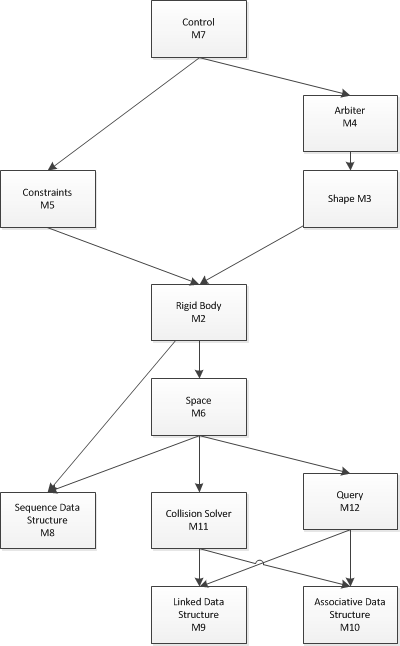
\includegraphics[width=0.75\textwidth]{uses.png}
}
\caption{\label{Fig_uses}Use hierarchy among Modules}
\end{center}
\end{figure}


\section{Inheritance Hierarchy Between Modules} \label{SecInheritance}
In this section the inheritance hierarchy between modules is provided(Figure \ref{Fig_Inheritance}).
Modules in the lower level of the hierarchy inherit properties from the higher levels.
\begin{figure}[htbp]
\begin{center}
%\rotatebox{-90}
{
 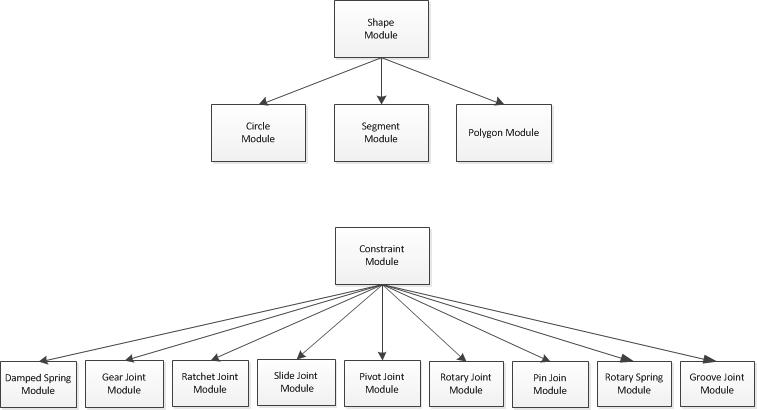
\includegraphics[width=1\textwidth]{inherit.png}
}
\caption{\label{Fig_Inheritance}Inheritance hierarchy among Modules}
\end{center}
\end{figure}


%\section*{References}

\bibliography {Game Physics Library MG}{}
\bibliographystyle {plain}

\end{document}